\documentclass[french]{article}
\usepackage[T1]{fontenc}
\usepackage[utf8]{inputenc}
\usepackage[french]{babel}
\usepackage{amsmath}
\usepackage{mathtools}
\usepackage{color}
\usepackage[svgnames,dvipsnames]{xcolor} 
\usepackage{soul}
\usepackage{amssymb}
\usepackage{enumitem}
\usepackage{multicol}
\usepackage[left=2cm,right=2cm,top=2cm,bottom=2cm]{geometry}
\newcommand{\mathcolorbox}[2]{\colorbox{#1}{$\displaystyle #2$}}
\usepackage{pifont}
\usepackage{pst-all}
\usepackage{pstricks}
\usepackage{delarray}
\usepackage{setspace}
\usepackage{graphicx}
\usepackage{hyperref}
\usepackage{nicematrix}
\usepackage{listings}
\usepackage{float}

\hypersetup{
	colorlinks=true,
	linkcolor=blue,
	filecolor=magenta,      
	urlcolor=cyan,
	pdftitle={Overleaf Example},
	pdfpagemode=FullScreen,
}

\usepackage{amsthm}
\newtheorem*{Rem}{Remarque}

\newenvironment{conclusion}[1]{%
	\begin{center}\normalfont\textbf{Conclusion}\end{center}
	\begin{quotation} #1 \end{quotation}
}{%
	\vspace{1cm}
}

\lstset{language=C++,
	basicstyle=\ttfamily,
	keywordstyle=\color{blue}\ttfamily,
	stringstyle=\color{red}\ttfamily,
	commentstyle=\color{green}\ttfamily,
	morecomment=[l][\color{magenta}]{\#}
}

\begin{document}
	LECOURTIER Frédérique \hfill \today
	\begin{center}
		\Large\textbf{{Extrapolate - FEniCS}}\\
	\end{center}
	\graphicspath{{images/}}

	Après plusieurs tests sur la partie de correction/certification du modèle où l'on prend la solution analytique comme nouvelle level-set, il semblerait que la méthode avec les meilleurs résultats soit celle où l'on utilise la méthode \textbf{extrapolate} de FEniCS. C'est pourquoi, on va ici présenter en détail le code source de cette fonction car la documentation FEniCS au sujet de cette méthode n'est pas très complète (\href{https://fenics.readthedocs.io/projects/dolfin/en/2017.2.0/apis/api_adaptivity.html#extrapolation}{Extrapolation}).
	
	Pour illustrer les explications, nous considérerons un domaine rectangulaire maillés uniformément par des triangles. Dans la suite, nous considérerons également \textit{cell0} comme étant une des cellules de maillage. On prendra comme exemple une extrapolation de $\mathbb{P}^1$ vers $\mathbb{P}^2$ : 
	
	\begin{minipage}{0.48\linewidth}
		\begin{figure}[H]
			\centering
			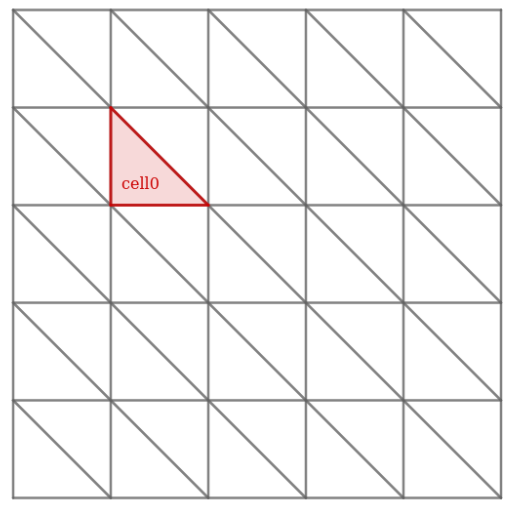
\includegraphics[width=0.5\linewidth]{cell0.png}
			\caption{Cell0}
		\end{figure}
	\end{minipage}
	\begin{minipage}{0.48\linewidth}
		\begin{figure}[H]
			\centering
			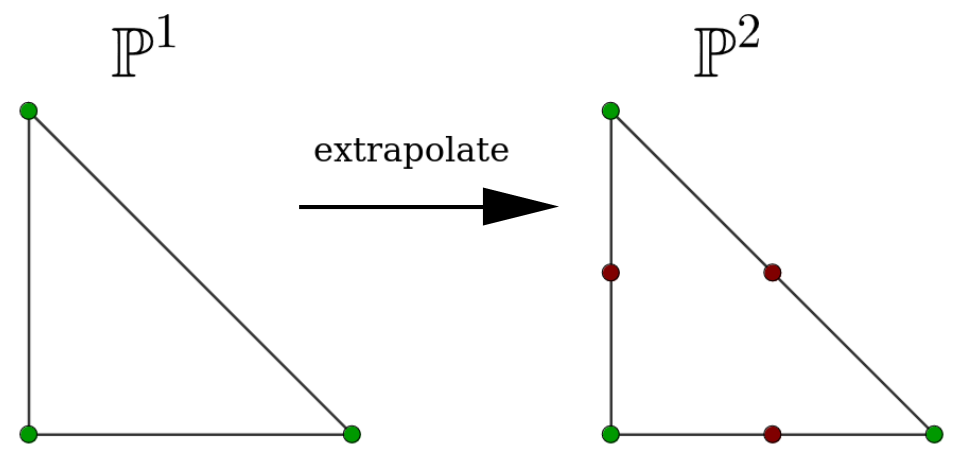
\includegraphics[width=0.9\linewidth]{P1toP2.png}
			\caption{Extrapolation de $\mathbb{P}^1$ vers $\mathbb{P}^2$}
		\end{figure}
	\end{minipage}
	
	\section{extrapolate}
	\label{extrapolate}
	
	Corps de la fonction :

	\begin{lstlisting}
void Extrapolation::extrapolate(Function& w, const Function& v)
	\end{lstlisting}
	
	Cette fonction a pour but d'extrapoler la fonction $v$ en une fonction $w$. \\
	
	On cherche à calculer la valeur en chacun des degrés de liberté associé à la fonction $w$. Pour cela, on va parcourir toutes les cellules du maillage dans le but de construire le tableau \textit{coefficients} (de taille le nombre total de degrés de liberté associés à $w$). On appelle alors sur chacune des cellules la fonction \textbf{compute\_coefficients}~\ref{compute_coefficients} qui va compléter le tableau \textit{coefficients} aux indices associées à ses degrés de liberté. Comme les degrés de liberté d'une cellule peuvent être communs à ceux d'une autre, on finira par faire une moyenne des coefficients en chacun des degrés de liberté, ce qui nous donne alors la fonction $w$. 
	
	\section{compute\_coefficients}
	\label{compute_coefficients}
	
	Corps de la fonction :
	
	\begin{lstlisting}
void Extrapolation::compute_coefficients(
  std::vector<std::vector<double>>& coefficients,
  const Function& v,
  const FunctionSpace& V,
  const FunctionSpace& W,
  const Cell& cell0,
  const std::vector<double>& coordinate_dofs0,
  const ufc::cell& c0,
  const Eigen::Ref<const Eigen::Matrix<dolfin::la_index, Eigen::Dynamic, 1>> dofs,
  std::size_t& offset)
	\end{lstlisting}
	
	Cette fonction a pour but de compléter le tableau \textit{coefficients} aux indices associées aux degrés de liberté d'une cellule donnée \textit{cell0}. \fbox{A COMPLETER !!!}
	
	
	
	\section{build\_unique\_dofs}
	\label{build_unique_dofs}
	
	Corps de la fonction :
	
	\begin{lstlisting}
void Extrapolation::build_unique_dofs(
  std::set<std::size_t>& unique_dofs,
  std::map<std::size_t, std::map<std::size_t, std::size_t>>& cell2dof2row,
  const Cell& cell0,
  const FunctionSpace& V)
	\end{lstlisting}

	Cette fonction a pour but de compléter les tableaux \textit{cell2dof2row} et \textit{unique\_dofs} donnés en entrée. Le set \textit{unique\_dofs} contient tous les degrés de liberté des cellules voisines à \textit{cell0}. Le dictionnaire \textit{cell2dof2row} permet d'associer à chaque degrés de liberté (unique) d'une cellule donné un numéro de ligne unique. Au total, on trouvera le même nombre de de degré de liberté dans \textit{cell2dof2row} et \textit{unique\_dofs}.\\
	
	On commence par remplir un set contenant les cellules voisines à \textit{cell0}. Pour être plus précis, les cellules voisines à \textit{cell0} sont les cellules ayant un nœud commun avec la cellule courante \textit{cell0} :
	\begin{figure}[H]
		\centering
		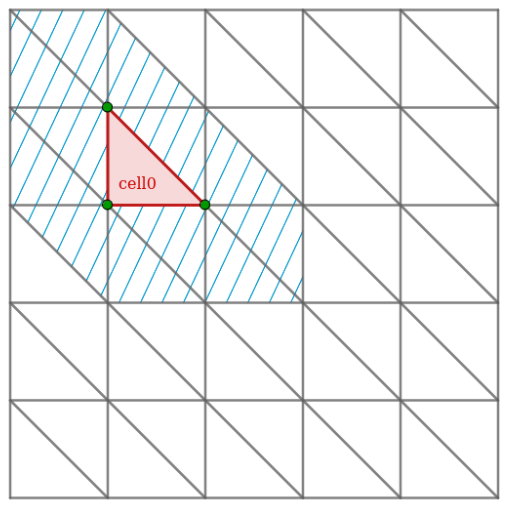
\includegraphics[width=0.25\linewidth]{surrounding_cells.png}
		\caption{Cellules voisines à Cell0}
	\end{figure}
	En parcourant ensuite chacune de ces cellules, on va pouvoir compléter les tableaux \textit{cell2dof2row} et \textit{unique\_dofs} donnés en entrée en appelant la fonction \textbf{compute\_unique\_dofs}~\ref{compute_unique_dofs}. \\
	Dans le cas de notre exemple, on va numéroter tous les nœuds des cellules voisines à \textit{cell0} de la manière suivante et on supposera que le parcours des cellules est effectuées dans l'ordre suivant :
	\begin{figure}[H]
		\centering
		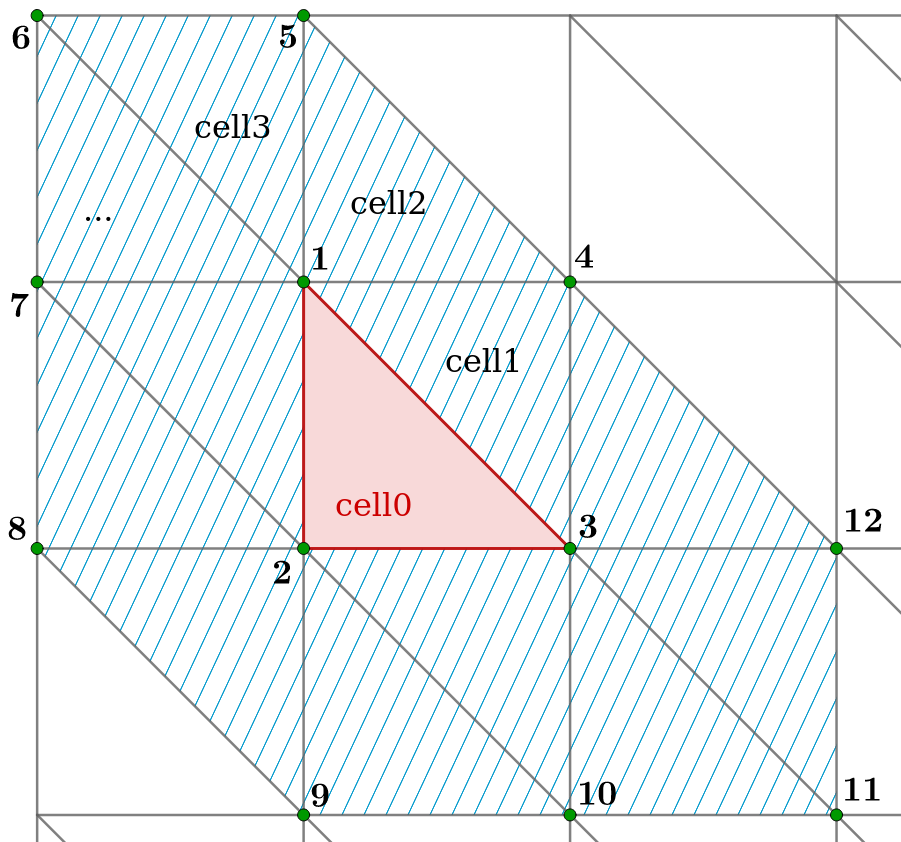
\includegraphics[width=0.25\linewidth]{cell2dof2row.png}
		\caption{Parcours des cellules voisines}
	\end{figure}
	Alors le set \textit{unique\_dofs} contiendra tous les noeuds des cellules voisines à \textit{cell0} : 
	$$unique\_dofs = \{1,2,3,\dots,12\}$$
	
	Et le dictionnaire \textit{cell2dof2row} associé à \textit{cell0} est construit de la manière suivante :
	$$cell2dof2row = \begin{aligned}[t]
		\{\quad&"cell0":\{"dof1":0,"dof2":1,"dof3":2\},&& \\
		&"cell1":\{"dof4":3\}, \\
		&"cell2":\{"dof5":4\}, \\
		&\dots &&\}
	\end{aligned}$$
	
	
	\section{compute\_unique\_dofs}
	\label{compute_unique_dofs}
	
	Corps de la fonction :
	
	\begin{lstlisting}
std::map<std::size_t, std::size_t> Extrapolation::compute_unique_dofs(
  const Cell& cell,
  const FunctionSpace& V,
  std::size_t& row,
  std::set<std::size_t>& unique_dofs)
	\end{lstlisting}
	
	Cette fonction a pour but de traiter chacune des cellules voisines afin de compléter les tableaux \textit{unique\_dofs} et \textit{cell2dof2row} créés dans \textbf{build\_unique\_dofs}~\ref{build_unique_dofs}.\\
	
	Pour une cellule \textit{cell} (voisine à \textit{cell0}), on va parcourir chacun de ses degrés de liberté associé à l'espace $V$. Autrement dit, on parcourt tous les degrés de liberté dont la valeur est connue (dans notre cas les degrés de liberté $\mathbb{P}^1$ et donc les noeuds de la cellule). Si ce degré de liberté fait partie de \textit{unique\_dofs}, on ne fait rien. Sinon, on l'ajoute à \textit{unique\_dofs}. On va également créer un tableau \textit{dof2row} qui a pour but d'associer un degré de liberté à un numéro de ligne unique. Ce dictionnaire \textit{dof2row} est retourné par la fonction et permet de remplir le dictionnaire plus général \textit{cell2dof2row} créé dans \textbf{build\_unique\_dofs}~\ref{build_unique_dofs}.
	
	\section{add\_cell\_equations}
	\label{add_cell_equations}
	
	\section{average\_coefficients}
	\label{average_coefficients}

	\newpage
	\appendix
	
	\section{Code source FEniCS}
	
	\lstinputlisting[language=C++]{Extrapolation.cpp}
	
\end{document}